\documentclass{article}
\usepackage{PRIMEarxiv}
\usepackage[utf8]{inputenc} % allow utf-8 input
\usepackage[T1]{fontenc}    % use 8-bit T1 fonts
\usepackage{palatino,eulervm}
\usepackage{hyperref}       % hyperlinks
\usepackage{url}            % simple URL typesetting
\usepackage{booktabs}       % professional-quality tables
\usepackage{amsfonts}       % blackboard math symbols
\usepackage{nicefrac}       % compact symbols for 1/2, etc.
\usepackage{microtype}      % microtypography
\usepackage{lipsum}
\usepackage{fancyhdr}       % header
\usepackage{graphicx}       % graphics
\graphicspath{{media/}}     % organize your images and other figures under media/ folder
\usepackage{minted}

\pagestyle{fancy}
\thispagestyle{empty}
\rhead{ \textit{ }} 

\fancyhead[LO]{SVD Factorization for Tall-and-Fat Matrices on Paralel Architectures}
  
\title{SVD Factorization for Tall-and-Fat Matrices on Paralel Architectures}

\author{
  Burak Bayramlı \\
  İstanbul, Turkey\\
  \texttt{burakbayramli.github.io} 
}


\begin{document}

\maketitle

\begin{abstract}
We demonstrate an implementation for an approximate rank-k SVD factorization,
combining well-known randomized projection techniques with previously known
paralel solutions in order to compute steps of the random projection based SVD
procedure. We structure the problem in a way that it reduces to fast computation
around $k \times k$ matrices computed on a single machine, greatly easing the
computability of the problem. The paper is also a tutorial on paralel linear
algebra methods using a plain architecture without burdensome frameworks.
\end{abstract}


% keywords can be removed
\keywords{Parallel \and Concurrency \and Big Data}

\section{Introduction}

\section{Headings: first level}
\label{sec:headings}

\lipsum[4] See Section \ref{sec:headings}.

\subsection{Headings: second level}
\lipsum[5]
\begin{equation}
\xi _{ij}(t)=P(x_{t}=i,x_{t+1}=j|y,v,w;\theta)= {\frac {\alpha _{i}(t)a^{w_t}_{ij}\beta _{j}(t+1)b^{v_{t+1}}_{j}(y_{t+1})}{\sum _{i=1}^{N} \sum _{j=1}^{N} \alpha _{i}(t)a^{w_t}_{ij}\beta _{j}(t+1)b^{v_{t+1}}_{j}(y_{t+1})}}
\end{equation}

\subsubsection{Headings: third level}
\lipsum[6]

\paragraph{Paragraph}
\lipsum[7]

\section{Implementation}

Big Data became possible largely thanks to Map/Reduce architectures which
represent splitting (mapping) and grouping (reducing) concepts logically and
present them the only interface for a programmer to worry about, while in the
background directing data pieces produced by mapping and reducing to appropiate
seperate nodes to achieve concurrency. A sample process is seen in
Figure~\ref{fig:mapreduce1},

\begin{figure}[h]
  \centering
  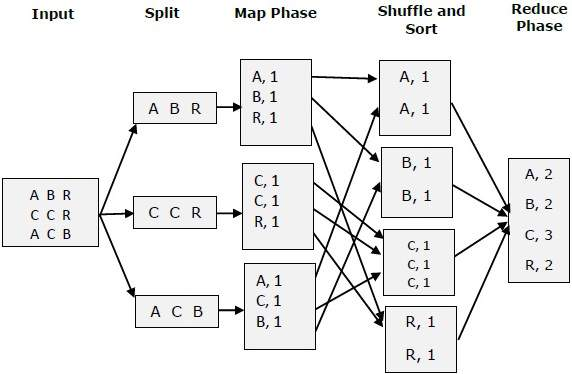
\includegraphics[width=20em]{mapreduce1.jpg}
  \caption{Example Map Reduce Process}
  \label{fig:mapreduce1}
\end{figure}

\subsection{Architecture}

\begin{minted}[fontsize=\footnotesize]{python}
import os, numpy as np

def process(file_name,N,hookobj):
    file_size = os.path.getsize(file_name)
    beg = 0
    chunks = []
    for i in range(N):
        with open(file_name, 'r') as f:
            s = int((file_size / N)*(i+1))
            f.seek(s)
            f.readline()
            end_chunk = f.tell()-1
            chunks.append([beg,end_chunk])
            f.close()
        beg = end_chunk+1
    c = chunks[hookobj.ci]
    with open(file_name, 'r') as f:
        f.seek(c[0])
        while True:
            line = f.readline()
            hookobj.exec(line)
            if f.tell() > c[1]: break
        f.close()
        hookobj.post()
\end{minted}






\label{sec:others}
\lipsum[8] \cite{kour2014real,kour2014fast} and see \cite{hadash2018estimate}.

The documentation for \verb+natbib+ may be found at
\begin{center}
  \url{http://mirrors.ctan.org/macros/latex/contrib/natbib/natnotes.pdf}
\end{center}
Of note is the command \verb+\citet+, which produces citations
appropriate for use in inline text.  For example,
\begin{verbatim}
   \citet{hasselmo} investigated\dots
\end{verbatim}
produces
\begin{quote}
  Hasselmo, et al.\ (1995) investigated\dots
\end{quote}

\begin{center}
  \url{https://www.ctan.org/pkg/booktabs}
\end{center}


\subsection{Figures}
\lipsum[10] 
See Figure \ref{fig:fig1}. Here is how you add footnotes. \footnote{Sample of the first footnote.}
\lipsum[11] 

\subsection{Tables}
\lipsum[12]
See awesome Table~\ref{tab:table}.

\begin{table}
 \caption{Sample table title}
  \centering
  \begin{tabular}{lll}
    \toprule
    \multicolumn{2}{c}{Part}                   \\
    \cmidrule(r){1-2}
    Name     & Description     & Size ($\mu$m) \\
    \midrule
    Dendrite & Input terminal  & $\sim$100     \\
    Axon     & Output terminal & $\sim$10      \\
    Soma     & Cell body       & up to $10^6$  \\
    \bottomrule
  \end{tabular}
  \label{tab:table}
\end{table}

\subsection{Lists}
\begin{itemize}
\item Lorem ipsum dolor sit amet
\item consectetur adipiscing elit. 
\item Aliquam dignissim blandit est, in dictum tortor gravida eget. In ac rutrum magna.
\end{itemize}


\section{Conclusion}
Your conclusion here

\section*{Acknowledgments}
This was was supported in part by......

%Bibliography
\bibliographystyle{unsrt}  

\begin{thebibliography}{1}

\bibitem{gleich}
Gleich, Benson, Demmel, \emph{Direct QR factorizations for tall-and-skinny
  matrices in MapReduce architectures}, {\tt arXiv:1301.1071 [cs.DC]}, 2013

\bibitem{halko}
N.~Halko, \emph{Randomized methods for computing low-rank approximations of
  matrices}, University of Colorado, Boulder, 2010

\bibitem{gupta}
S.~Dangupta, A.~Gupta \emph{An Elementary Proof of a Theorem of Johnson and
  Lindenstrauss}, Wiley Periodicals, 2002

\bibitem{kurucz}
M.~Kurucz, A. A.~Benczúr, K.~Csalogány, \emph{Methods for large scale SVD with
missing values}, ACM, 2007

\bibitem{zadeh}
Zadeh, \emph{CME 323: Distributed Algorithms and Optimization, Lecture 17}, 
\url{https://stanford.edu/~rezab/classes/cme323/S17/}
  
\end{thebibliography}

\end{document}
